\documentclass[a4paper]{article}
%\documentclass[8pt]{report}
%%%%%%%% CREATE DOCUMENT STRUCTURE %%%%%%%%
%% Language and font encodings
\usepackage[english]{babel}
\usepackage[utf8x]{inputenc}
\usepackage[T1]{fontenc}

%\usepackage{subfig}

%% Sets page size and margins
\usepackage[a4paper,top=3cm,bottom=2cm,left=2cm,right=2cm,marginparwidth=1.75cm]{geometry}

%% Useful packages
\usepackage{amsmath}
\usepackage{graphicx}
\usepackage[colorinlistoftodos]{todonotes}
\usepackage[colorlinks=true, allcolors=blue]{hyperref}
%\usepackage{caption}
\usepackage[justification=centering]{caption}
\usepackage{subcaption}
\usepackage{sectsty}
\usepackage{float}
\usepackage{titling} 
\usepackage{blindtext}
\usepackage[square,sort,comma,numbers]{natbib}
\usepackage[colorinlistoftodos]{todonotes}
\usepackage{xcolor}
\usepackage{fancyhdr}
\usepackage{lipsum}

%% definitions 
\definecolor{darkgreen}{rgb}{0.0, 0.4, 0.0}

%% Define your personal info here %%%%%%%%%%%%%%%%%%%%%%%
\newcommand\TPid{1}
\newcommand\TPname{Graphical rdfs - Marché de Carouge}
\newcommand\Firstname{Joao Filipe}
\newcommand\Familyname{Costa da Quinta}
\newcommand\Email{Joao.Costa@etu.unige.ch}
\newcommand\Firstnames{Léa}
\newcommand\Familynames{Heiniger}
\newcommand\Emails{Lea-Marie.Heiniger@etu.unige.ch}

%%%%%%%%%%%%%%%%%%%%%%%%%%%%%%%%%%%%%%%%%%%%%%%%%%%%%%%

%%%%%%% Page header %%%%%%
\pagestyle{fancy}
\fancyhf{}
\rhead{TP \TPid: \TPname}
\lhead{\Firstnames \ \Familynames , \ \Firstname \ \Familyname}
\rfoot{Page \thepage}


%%%%%%%% DOCUMENT %%%%%%%%
\begin{document}

%%%% Title Page
\begin{titlepage}

\newcommand{\HRule}{\rule{\linewidth}{0.5mm}} 							% horizontal line and its thickness

\center 
 
% University
\textsc{\LARGE Université de Genève}\\[1cm]

% Document info
\textsc{\Large Technologies du web sémantique}\\[0.2cm]									% Course Code
\HRule \\[0.8cm]
{ \huge \bfseries TP \TPid : \TPname}\\[0.7cm]								% Assignment
\HRule \\[2cm]
\large
\emph{Author:} \Firstnames \  \Familynames\\[0.5cm]		
\emph{E-mail:} {\color{blue}\Emails}\\[0.5cm]
\emph{Author:} \Firstname \  \Familyname\\[0.5cm]		
\emph{E-mail:} {\color{blue}\Email}\\[6cm]	

% Author info
% Author info
{\large \today}\\[2cm]

\includegraphics[width=0.4\textwidth]{images/unige_csd.png}\\[1cm] 	% University logo
\vfill 
\end{titlepage}


% ============================================
% ----------------------------------
\newpage
\section*{Introduction}
The goal of this project is to make a description of a tourist area using URI data. To do this we must integrate data from various sources, mainly Open Street Map and DBpedia.\\\\

\subsection*{Selected Area}
For this project we choose, Place du Marché Carouge. This a location that is full of life and incredible locations of leisure, there are very nice cafés, bars, restaurants and even a cinema. This locations is also very well located in the heart of the Commune de Carouge in Geneva, and it has near access to public transportation, so that anyone can access it easily. \\\\ For more detailed overview of the attractions of Place du Marché Carouge, one simply has to see the initial RDF schema in the next section !

\subsection*{Initial RDF schema}
\begin{figure}[H]
\center
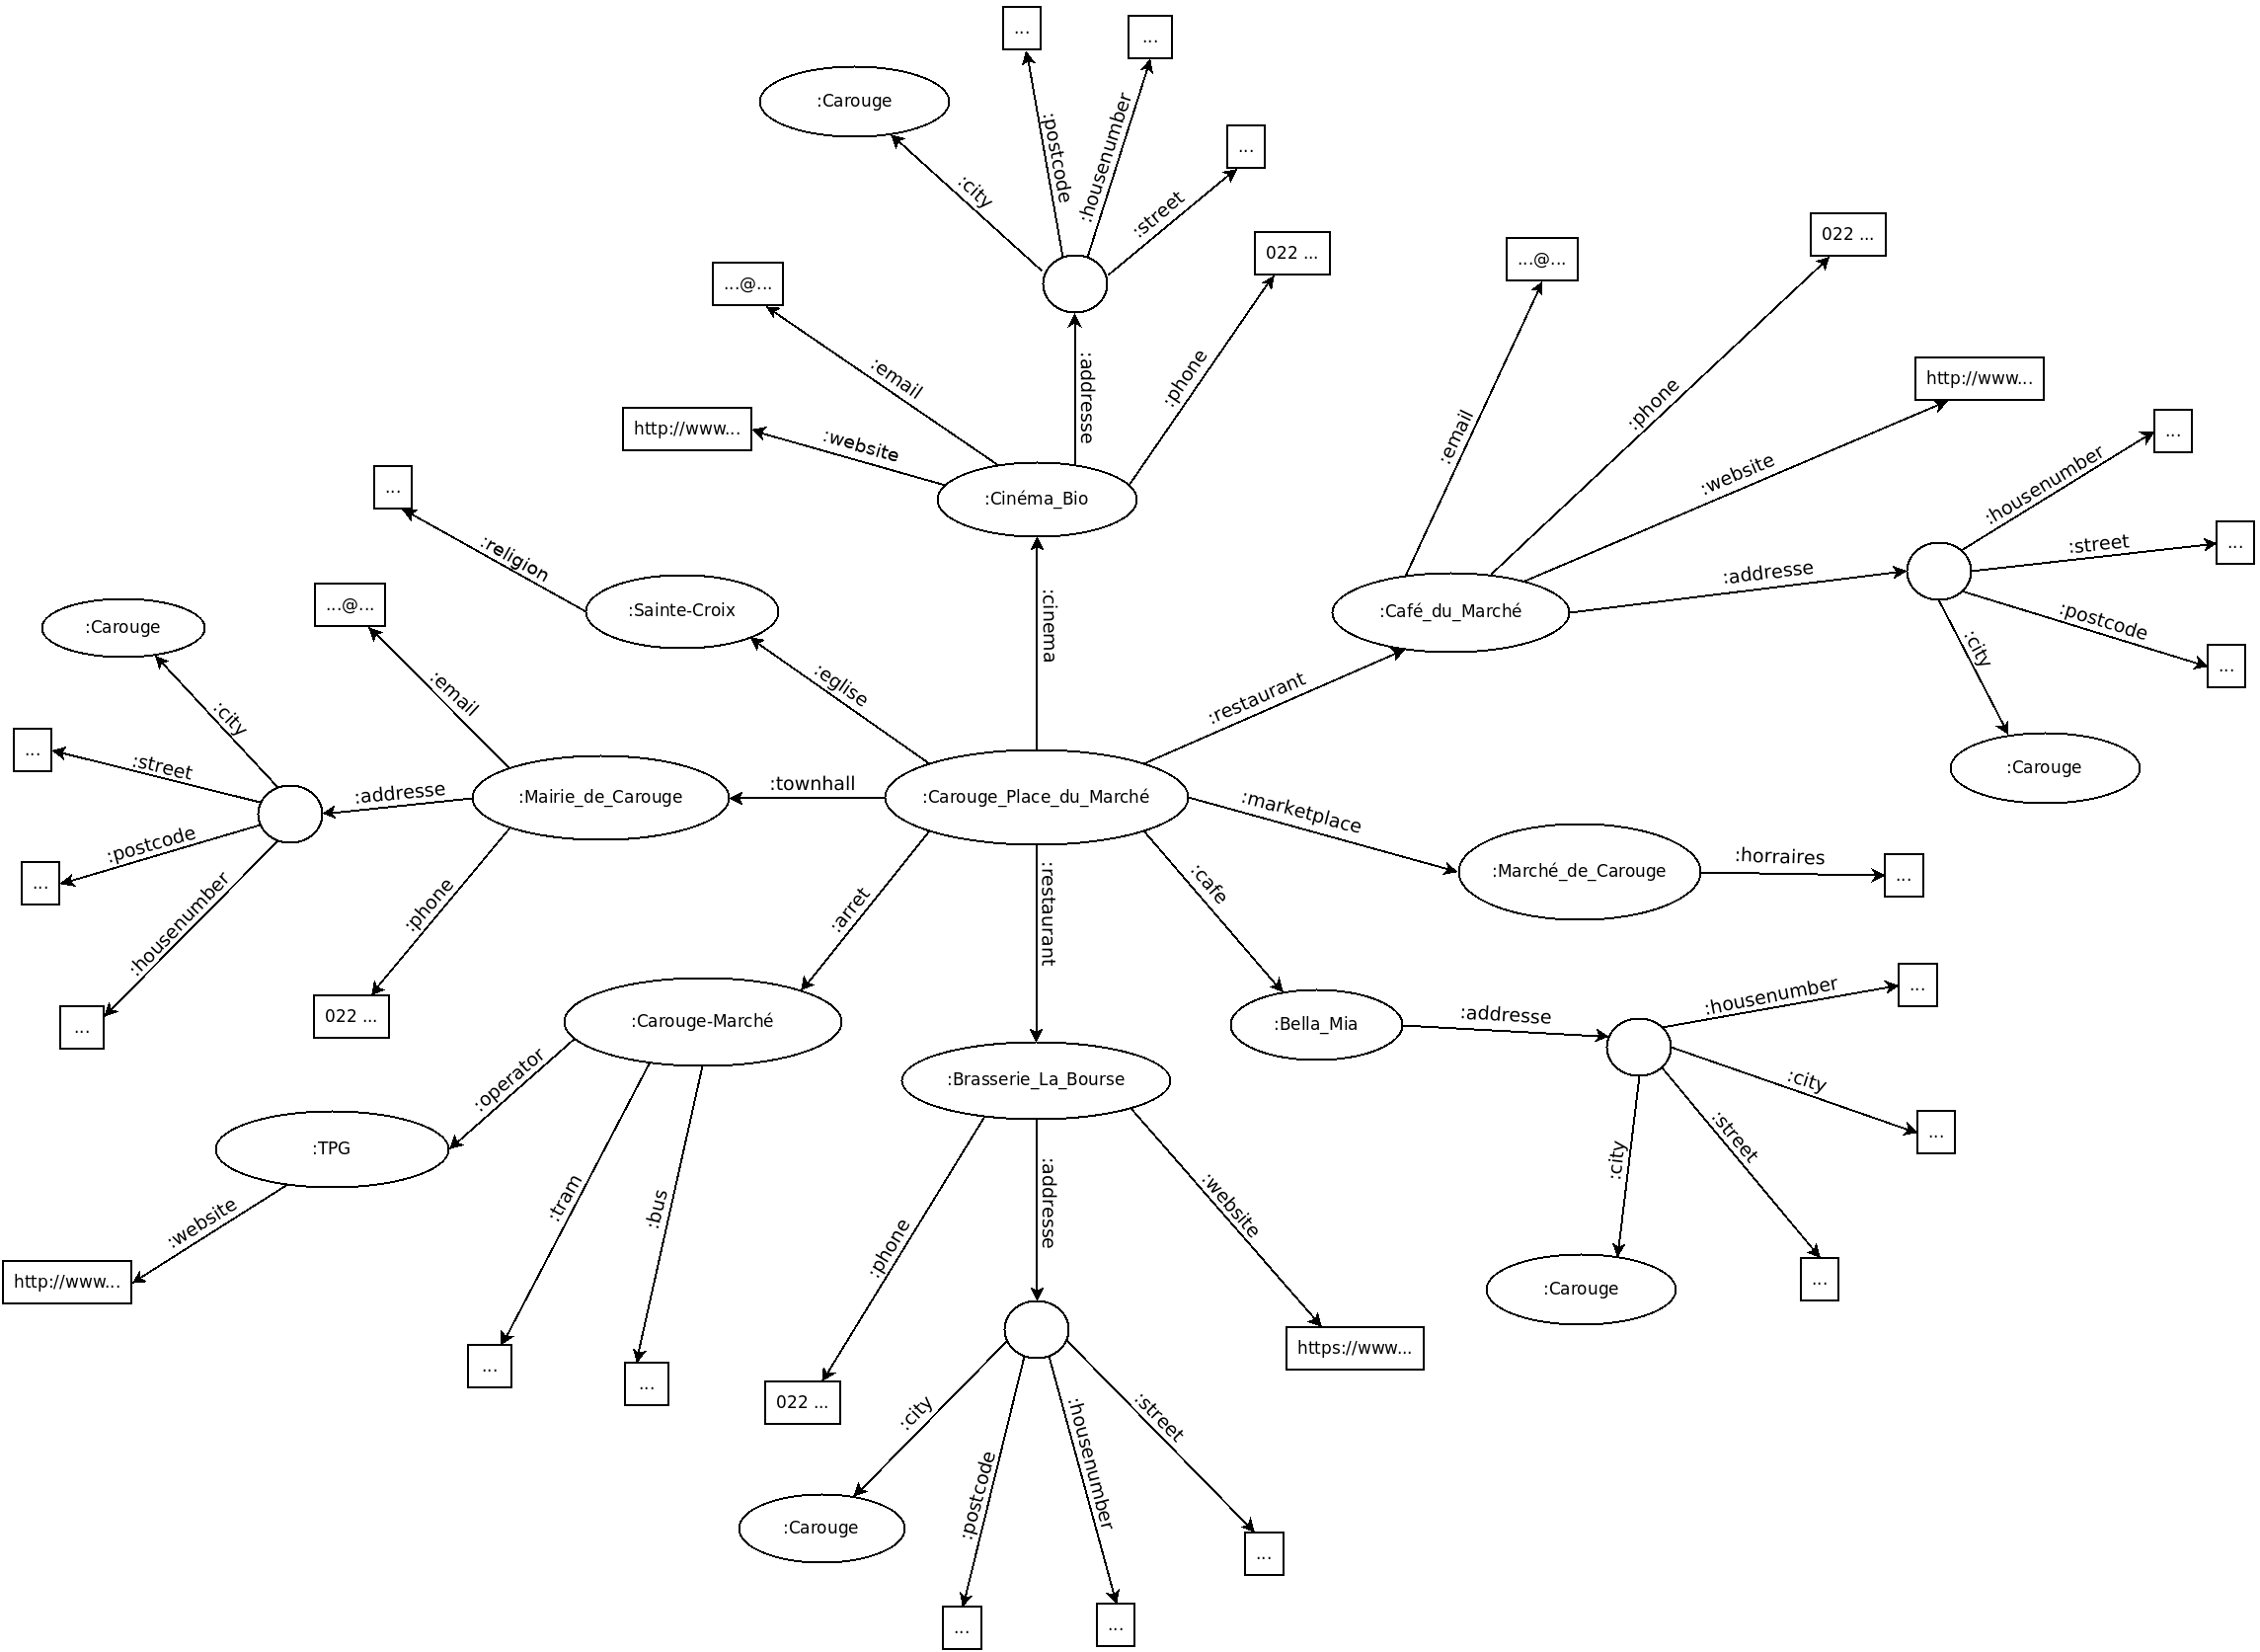
\includegraphics[width=1.1\textwidth]{images/Graph_init.PNG}
\caption{Initial RDF schema}
\end{figure}
\section*{Data sources}
To get all of the required information, we used OSM, which actually was full of information about the location we choose, this made our job easier, as we didn't have very large data to integrate from different sources. Any gaps that were left, were filled by using DBPedia, as well as the official web site of the Ville de Carouge.\\\\ With all three sources together we were able to fill our initial RDF schema with information.

\begin{figure}[H]
\center
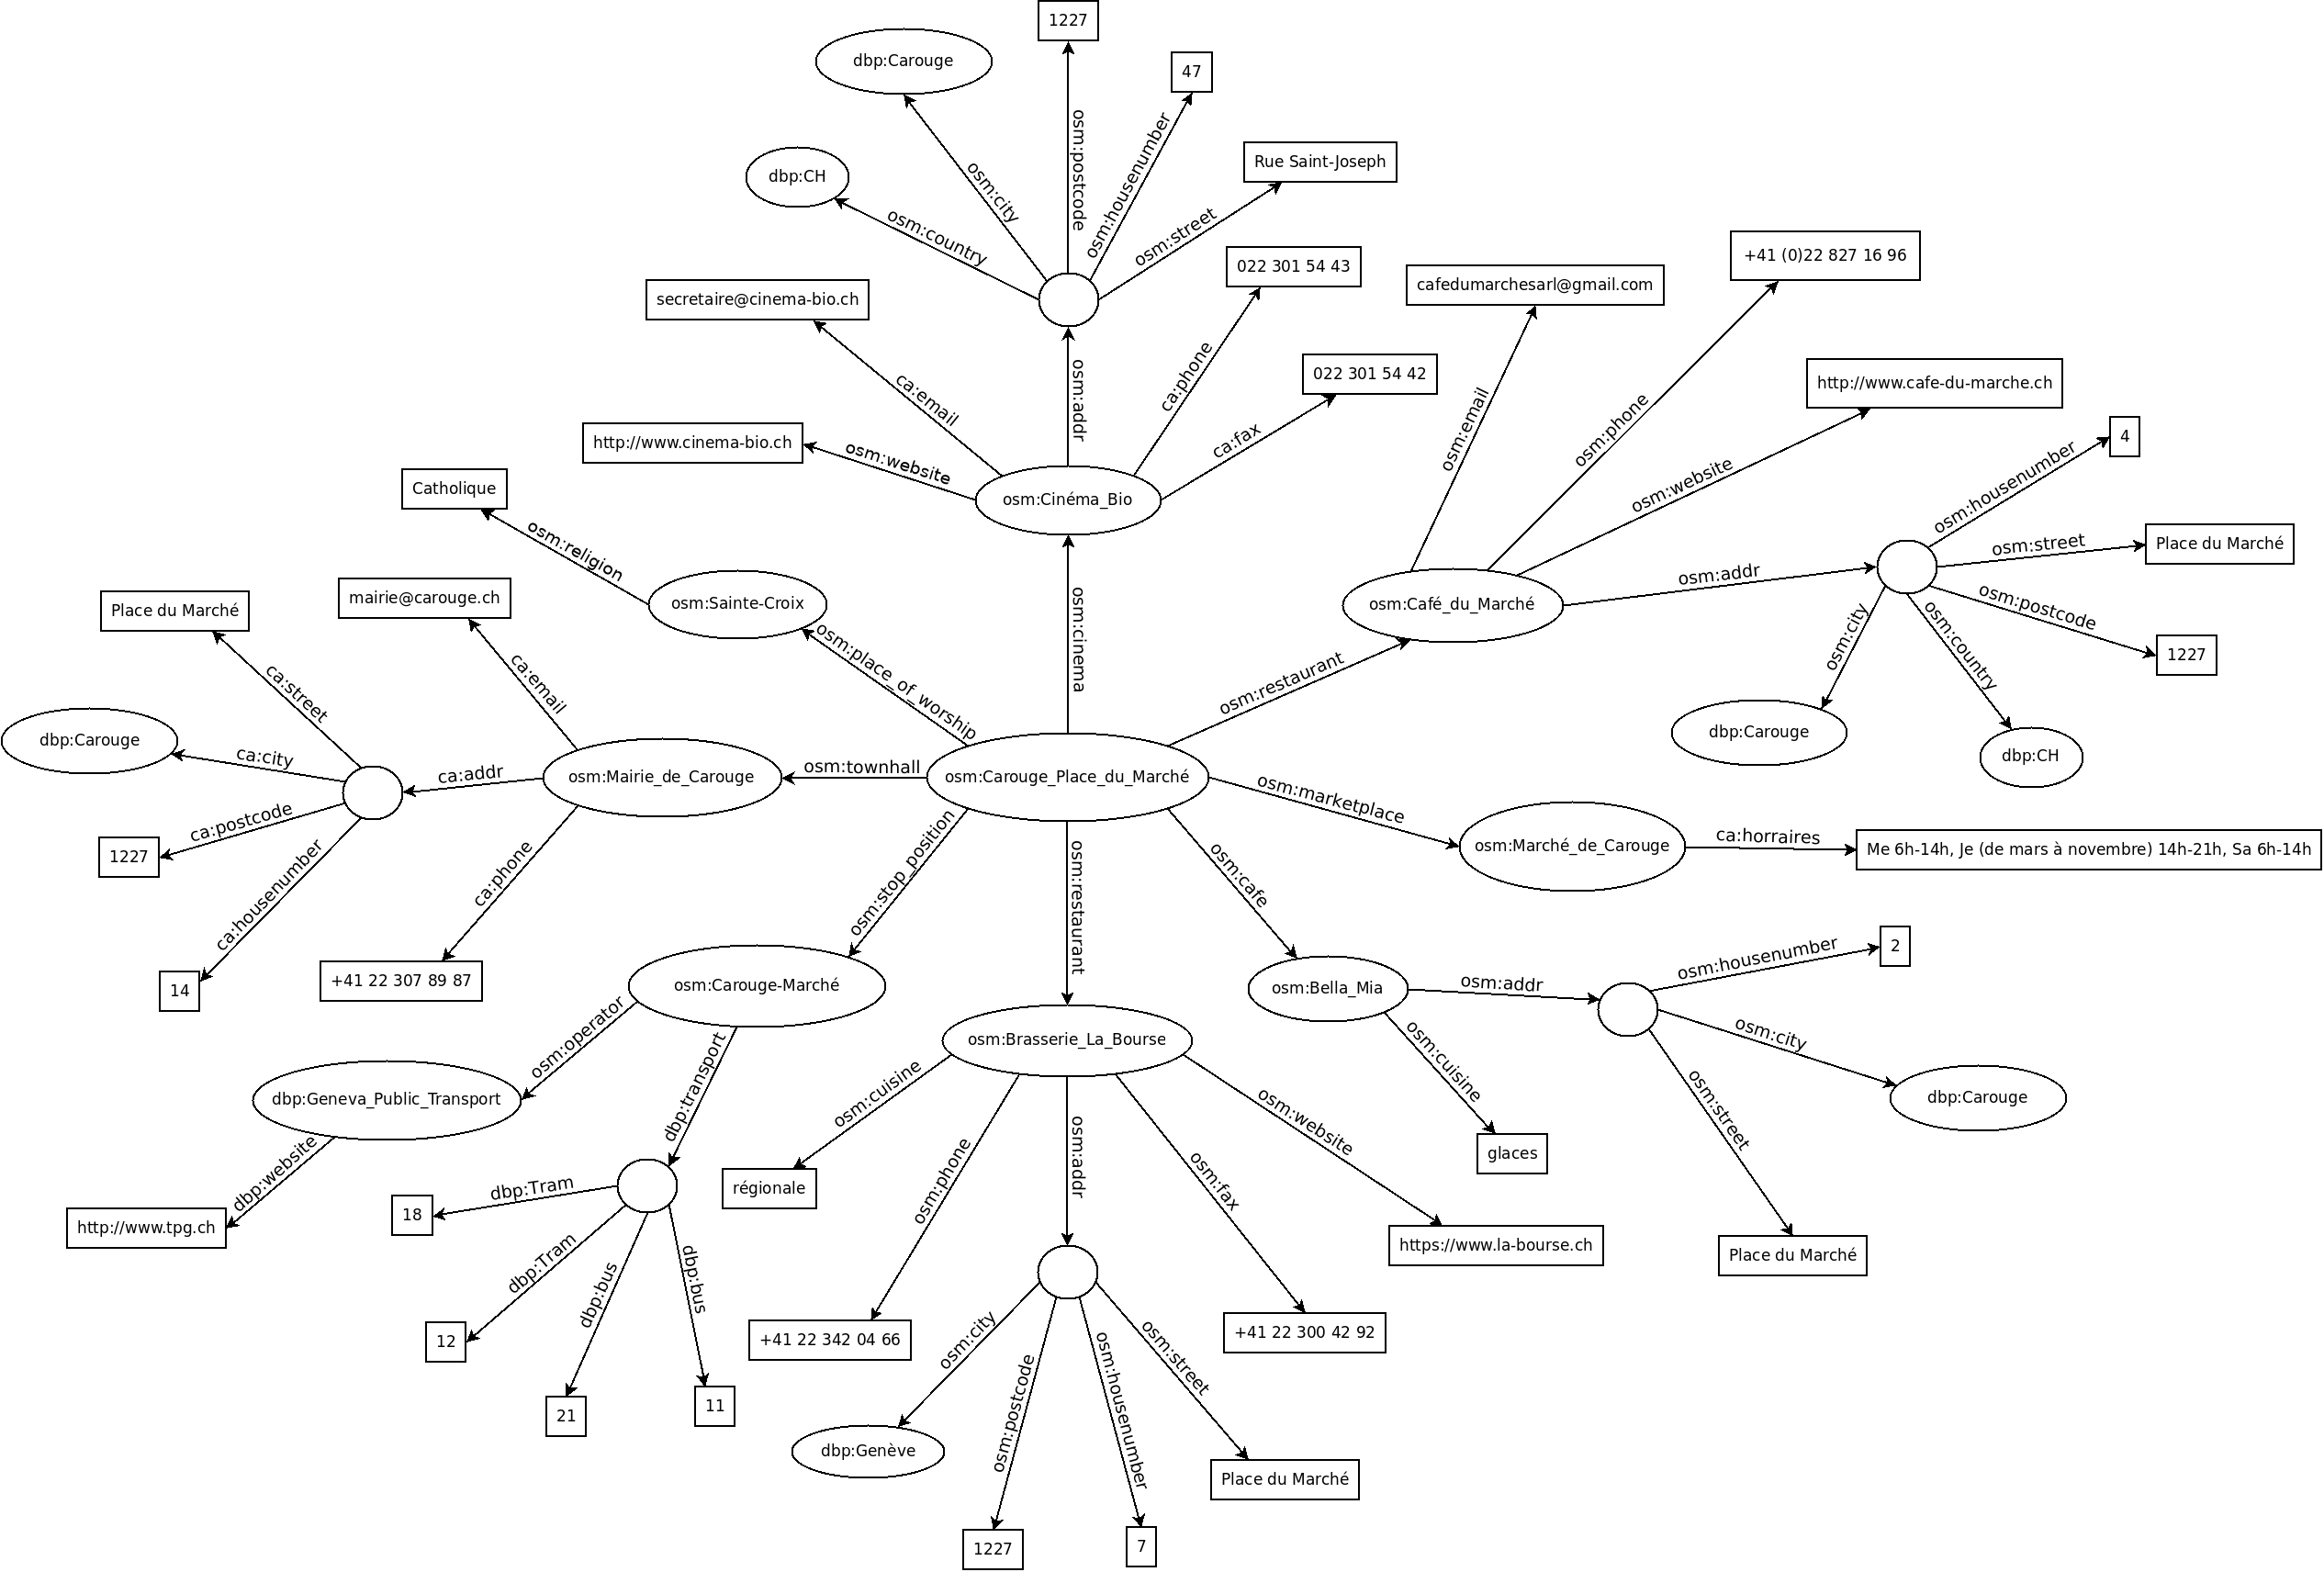
\includegraphics[width=1.1\textwidth]{images/Graph.PNG}
\caption{Final RDF Graph with all the data}
\end{figure}

\section*{GraphDB}
As our data was mostly in .osm, we created a turtle file where we input every information necessary for the construction of our graph, this exact file will be turned in as well, so you can easily see the organisation of the file. \\\\
With the file done we only needed to import the data to GraphDB. To visualize our graph we decided to go with a fixed center node, this node being the chosen tourist location. Here is our Graph :

\begin{figure}[H]
\center
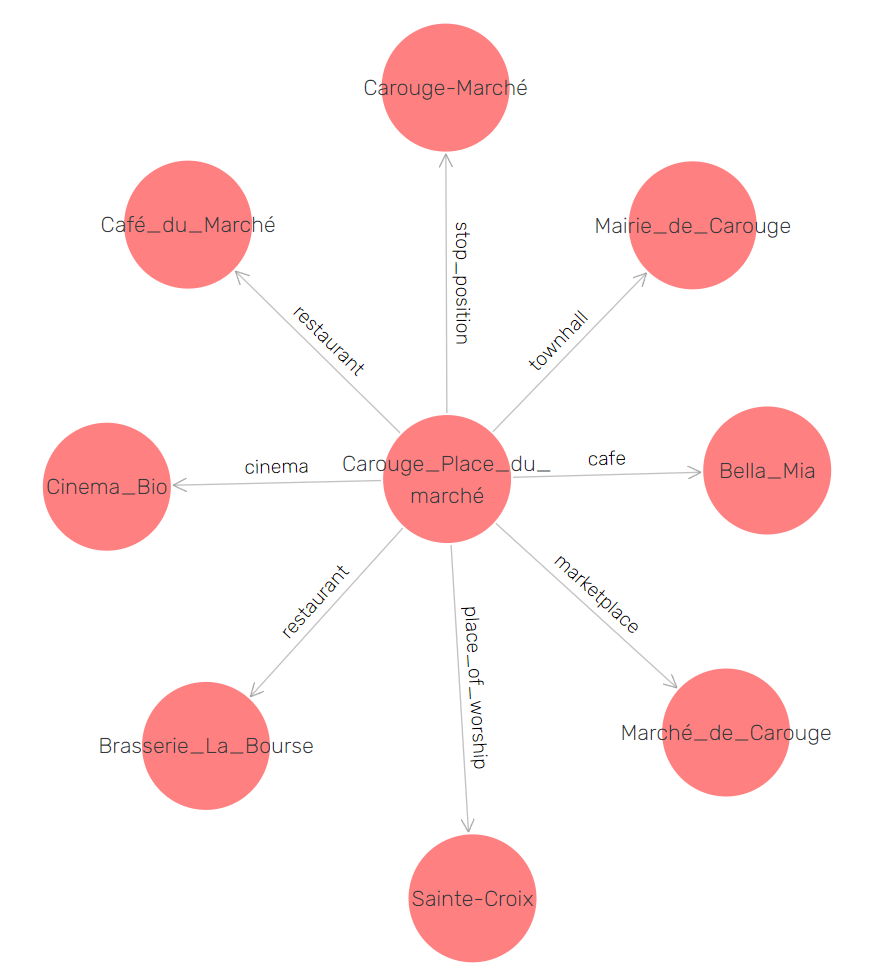
\includegraphics[width=0.8\textwidth]{images/Graph_graphdb.PNG}
\caption{Final RDF Graphin GraphDB}
\end{figure}
In this graph we can only see the immediate triplets to the center of the graph, however to get all information we need only to click a node, and all information will be displayed.

\newpage
\section*{SPARQL Query}
To show that our data is organised as intended as well as usable, one has to go no further than to do some SPARQL queries. SPARQL queries are used to get answers from a certain graph, in the same way one would use SQL queries to query a database. To use SPARQL we have to know its semantic rules, let's see some queries in action.\\\\

\subsection*{Hmm, what are the restaurants in the area ?}
Let's assume a tourist in the area wants to see which restaurants are available, he has only to query our graph to get some answers.
\begin{figure}[H]
\center
\includegraphics*[width=0.8\textwidth]{images/restaurant_query.PNG}
\caption{Query to ask for restaurants in the location}
\end{figure}
Because there are three different possible sources of restaurants, we must include all of them in the Query. This query results in the following : 
\begin{figure}[H]
\center
\includegraphics*[width=0.5\textwidth]{images/restaurant_query_res.PNG}
\caption{Result of query to ask for restaurants in the location}
\end{figure}
We can easily check the result by checking the RDF graph in the previous section.

\newpage
\subsection*{Hmm, how do we reach Cinema Bio}
Let's assume a tourist in the area wants the contact and location of Cinema Bio.
\begin{figure}[H]
\center
\includegraphics*[width=0.7\textwidth]{images/cinema_query.PNG}
\caption{Query to ask for data about Cinema Bio}
\end{figure}
This query results in the following : 
\begin{figure}[H]
\center
\includegraphics*[width=0.4\textwidth]{images/cinema_query_res.PNG}
\caption{Result of query to ask for data about Cinema Bio}
\end{figure}
We must do one additional Query, as the osm:addr is a blank node that might be the origin point of more triplets.
\begin{figure}[H]
\center
\includegraphics*[width=0.7\textwidth]{images/cinema2_query.PNG}
\caption{Query that returns the actual address of Cinema Bio}
\end{figure}
\begin{figure}[H]
\center
\includegraphics*[width=0.4\textwidth]{images/cinema2_query_res.PNG}
\caption{Result of query that returns the actual address of Cinema Bio}
\end{figure}
We can easily check the result by checking the RDF graph in the previous section.

\newpage
\subsection*{Hmm, what are the points of interest of a given street}
Let's assume a tourist in the area wants know what points of interest are in a given street, he has only to query our graph to get some answers.
\begin{figure}[H]
\center
\includegraphics*[width=0.8\textwidth]{images/place_rue_query.PNG}
\caption{Query to ask for points of interest in the street Place du Marché}
\end{figure}
Because there are three different possible sources of restaurants, we must include all of them in the Query. This query results in the following : 
\begin{figure}[H]
\center
\includegraphics*[width=0.5\textwidth]{images/place_rue_query_res.PNG}
\caption{Result of query to ask for points of interest in the street Place du Marché}
\end{figure}
We can easily check the result by checking the RDF graph in the previous section.
\end{document}
